\section*{Question 1}
Meet, from left to right, Joe, William, Jack and Averell, villains of our childhood that go by the name of the Dalton brothers. These inseparable brothers have a special rule among themselves. They always stand in order of their height.

Write a program \texttt{Daltons.java} that takes names of the brothers as command-line arguments and prints \texttt{false} unless the order in which arguments are given follows \textit{The Dalton Rule}.

Example:\\
\texttt{\% java TheDaltons Joe William Jack Averell > true}\\
\texttt{\% java TheDaltons Averell Jack William Joe > true}\\
\texttt{\% java TheDaltons Averell William Joe Jack > false}
\begin{figure}[H]\centering
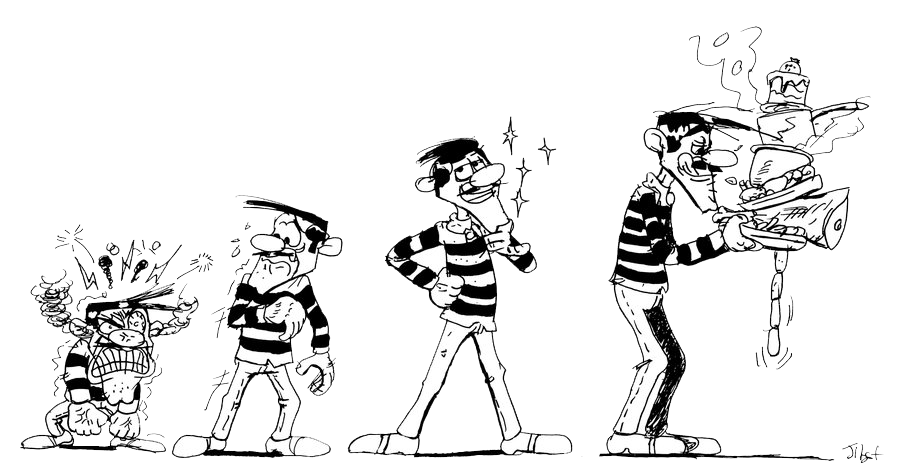
\includegraphics[width=10cm]{\topDirectory/template/images/daltons.png}
\caption{The Dalton Brothers}\label{fig1}
\end{figure}
\subsection*{Solution}
\lstset{language=Java}
\begin{lstlisting}
public class Daltons {
	public static void main (String[] args) {
		boolean result = false;
		// Check if brothers are from shortest to tallest
		if (args[0].equals("Joe") && args[1].equals("William") && args[2].equals("Jack") && args[3].equals("Averell")) {
			result = true;
		}
		// Check if brothers are from tallest to shortest
		else if (args[0].equals("Averell") && args[1].equals("Jack") && args[2].equals("William") && args[3].equals("Joe")) {
			result = true;
		}
		System.out.println(result);
	}
}
\end{lstlisting}
\section*{Question 2}
Matthew and John are playing backgammon and they hate rolling the two dice each turn, over and over again.
\begin{enumerate}
\item Write a program \texttt{Dice1.java} that gives two random integer numbers from one to six each time it is executed.
\item Upgrade your program to \texttt{Dice2.java} such that it takes an integer number as command-line argument and generates two random integer values in the range of one to given integer number.
\end{enumerate}
\subsection*{Solution}
\begin{lstlisting}
public class Dice1 {
	public static void main (String[] args) {
		// Generating two random numbers between 0 to 1
		double rand1 = Math.random();
		double rand2 = Math.random();
		// Convert range of random numbers and make them integers
		int randInt1 = (int) (6*rand1 + 1);
		int randInt2 = (int) (6*rand2 + 1);
		System.out.println(randInt1);
		System.out.println(randInt2);
	}
}
\end{lstlisting}
\begin{lstlisting}
public class Dice2 {
	public static void main (String[] args) {

		// Converting command-line argument to integer
		int maxNum = Integer.parseInt(args[0]);

		// Generating two random numbers between 0 to 1
		double rand1 = Math.random();
		double rand2 = Math.random();

		// Convert range of random numbers and make them integers
		int randInt1 = (int) (maxNum*rand1 + 1);
		int randInt2 = (int) (maxNum*rand2 + 1);
		System.out.println("First random number between 1 and " + maxNum + ": " + randInt1);
		System.out.println("Second random number between 1 and " + maxNum + ": " + randInt2);
	}
}
\end{lstlisting}
